\documentclass[twoside]{book}

% Packages required by doxygen
\usepackage{fixltx2e}
\usepackage{calc}
\usepackage{doxygen}
\usepackage[export]{adjustbox} % also loads graphicx
\usepackage{graphicx}
\usepackage[utf8]{inputenc}
\usepackage{makeidx}
\usepackage{multicol}
\usepackage{multirow}
\PassOptionsToPackage{warn}{textcomp}
\usepackage{textcomp}
\usepackage[nointegrals]{wasysym}
\usepackage[table]{xcolor}

% Font selection
\usepackage[T1]{fontenc}
\usepackage[scaled=.90]{helvet}
\usepackage{courier}
\usepackage{amssymb}
\usepackage{sectsty}
\renewcommand{\familydefault}{\sfdefault}
\allsectionsfont{%
  \fontseries{bc}\selectfont%
  \color{darkgray}%
}
\renewcommand{\DoxyLabelFont}{%
  \fontseries{bc}\selectfont%
  \color{darkgray}%
}
\newcommand{\+}{\discretionary{\mbox{\scriptsize$\hookleftarrow$}}{}{}}

% Page & text layout
\usepackage{geometry}
\geometry{%
  a4paper,%
  top=2.5cm,%
  bottom=2.5cm,%
  left=2.5cm,%
  right=2.5cm%
}
\tolerance=750
\hfuzz=15pt
\hbadness=750
\setlength{\emergencystretch}{15pt}
\setlength{\parindent}{0cm}
\setlength{\parskip}{3ex plus 2ex minus 2ex}
\makeatletter
\renewcommand{\paragraph}{%
  \@startsection{paragraph}{4}{0ex}{-1.0ex}{1.0ex}{%
    \normalfont\normalsize\bfseries\SS@parafont%
  }%
}
\renewcommand{\subparagraph}{%
  \@startsection{subparagraph}{5}{0ex}{-1.0ex}{1.0ex}{%
    \normalfont\normalsize\bfseries\SS@subparafont%
  }%
}
\makeatother

% Headers & footers
\usepackage{fancyhdr}
\pagestyle{fancyplain}
\fancyhead[LE]{\fancyplain{}{\bfseries\thepage}}
\fancyhead[CE]{\fancyplain{}{}}
\fancyhead[RE]{\fancyplain{}{\bfseries\leftmark}}
\fancyhead[LO]{\fancyplain{}{\bfseries\rightmark}}
\fancyhead[CO]{\fancyplain{}{}}
\fancyhead[RO]{\fancyplain{}{\bfseries\thepage}}
\fancyfoot[LE]{\fancyplain{}{}}
\fancyfoot[CE]{\fancyplain{}{}}
\fancyfoot[RE]{\fancyplain{}{\bfseries\scriptsize Generated by Doxygen }}
\fancyfoot[LO]{\fancyplain{}{\bfseries\scriptsize Generated by Doxygen }}
\fancyfoot[CO]{\fancyplain{}{}}
\fancyfoot[RO]{\fancyplain{}{}}
\renewcommand{\footrulewidth}{0.4pt}
\renewcommand{\chaptermark}[1]{%
  \markboth{#1}{}%
}
\renewcommand{\sectionmark}[1]{%
  \markright{\thesection\ #1}%
}

% Indices & bibliography
\usepackage{natbib}
\usepackage[titles]{tocloft}
\setcounter{tocdepth}{3}
\setcounter{secnumdepth}{5}
\makeindex

% Hyperlinks (required, but should be loaded last)
\usepackage{ifpdf}
\ifpdf
  \usepackage[pdftex,pagebackref=true]{hyperref}
\else
  \usepackage[ps2pdf,pagebackref=true]{hyperref}
\fi
\hypersetup{%
  colorlinks=true,%
  linkcolor=blue,%
  citecolor=blue,%
  unicode%
}

% Custom commands
\newcommand{\clearemptydoublepage}{%
  \newpage{\pagestyle{empty}\cleardoublepage}%
}

\usepackage{caption}
\captionsetup{labelsep=space,justification=centering,font={bf},singlelinecheck=off,skip=4pt,position=top}

%===== C O N T E N T S =====

\begin{document}

% Titlepage & ToC
\hypersetup{pageanchor=false,
             bookmarksnumbered=true,
             pdfencoding=unicode
            }
\pagenumbering{alph}
\begin{titlepage}
\vspace*{7cm}
\begin{center}%
{\Large C\+A\+Nflash }\\
\vspace*{1cm}
{\large Generated by Doxygen 1.8.13}\\
\end{center}
\end{titlepage}
\clearemptydoublepage
\pagenumbering{roman}
\tableofcontents
\clearemptydoublepage
\pagenumbering{arabic}
\hypersetup{pageanchor=true}

%--- Begin generated contents ---
\chapter{C\+A\+Nflash}
\label{md_README}
\Hypertarget{md_README}
Tool to use with C\+A\+Nloader. \section*{C\+A\+Nflasg}
\chapter{Todo List}
\label{todo}
\Hypertarget{todo}

\begin{DoxyRefList}
\item[\label{todo__todo000001}%
\Hypertarget{todo__todo000001}%
Global \hyperlink{canflash_8c_ae4dd3190f91742c0d6916aa0e251981c}{C\+A\+N\+\_\+init} (void)]Add other interfaces as K\+V\+A\+S\+ER leaf light 
\end{DoxyRefList}
\chapter{File Index}
\section{File List}
Here is a list of all files with brief descriptions\+:\begin{DoxyCompactList}
\item\contentsline{section}{inc/\hyperlink{canflash_8h}{canflash.\+h} }{\pageref{canflash_8h}}{}
\item\contentsline{section}{src/\hyperlink{canflash_8c}{canflash.\+c} }{\pageref{canflash_8c}}{}
\end{DoxyCompactList}

\chapter{File Documentation}
\hypertarget{canflash_8h}{}\section{inc/canflash.h File Reference}
\label{canflash_8h}\index{inc/canflash.\+h@{inc/canflash.\+h}}
{\ttfamily \#include $<$stdio.\+h$>$}\newline
{\ttfamily \#include $<$stdlib.\+h$>$}\newline
{\ttfamily \#include $<$stdint.\+h$>$}\newline
{\ttfamily \#include $<$string.\+h$>$}\newline
{\ttfamily \#include $<$unistd.\+h$>$}\newline
{\ttfamily \#include $<$canlib.\+h$>$}\newline
Include dependency graph for canflash.\+h\+:
\nopagebreak
\begin{figure}[H]
\begin{center}
\leavevmode
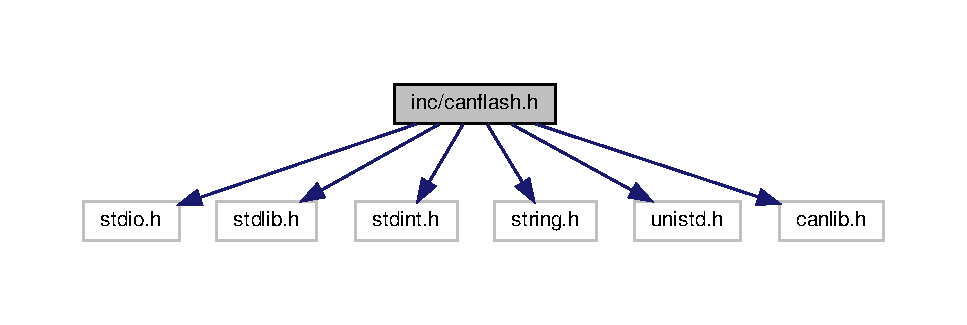
\includegraphics[width=350pt]{canflash_8h__incl}
\end{center}
\end{figure}
This graph shows which files directly or indirectly include this file\+:
\nopagebreak
\begin{figure}[H]
\begin{center}
\leavevmode
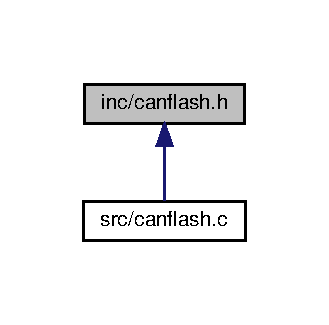
\includegraphics[width=158pt]{canflash_8h__dep__incl}
\end{center}
\end{figure}
\subsection*{Macros}
\begin{DoxyCompactItemize}
\item 
\#define \hyperlink{canflash_8h_aa9b3b183e3591e2dd08b8fe82a9066e5}{C\+A\+N\+\_\+\+C\+H\+A\+N\+N\+EL}~1
\item 
\#define \hyperlink{canflash_8h_a4d7374734c9286cabb8130d94e29af40}{C\+A\+N\+\_\+\+B\+L\+\_\+\+F\+L\+A\+S\+H\+ID}~0x\+AF
\item 
\#define \hyperlink{canflash_8h_aa75b7ce1cd135619656735399baf3768}{C\+A\+N\+\_\+\+B\+A\+U\+D\+R\+A\+TE}~can\+B\+I\+T\+R\+A\+T\+E\+\_\+250K
\end{DoxyCompactItemize}
\subsection*{Enumerations}
\begin{DoxyCompactItemize}
\item 
enum \hyperlink{canflash_8h_a3afab6089ad5eecc31a7f23ff17e5960}{C\+A\+N\+\_\+\+B\+L\+\_\+\+Type\+Def} \{ \newline
\hyperlink{canflash_8h_a3afab6089ad5eecc31a7f23ff17e5960aa6193fca03dc31ff466005ca57330ba8}{C\+A\+N\+\_\+\+B\+L\+\_\+\+OK} = 0x01, 
\hyperlink{canflash_8h_a3afab6089ad5eecc31a7f23ff17e5960a054ad8775ea84b7aacacd89d1610e952}{C\+A\+N\+\_\+\+B\+L\+\_\+\+C\+R\+C\+E\+RR} = 0x02, 
\hyperlink{canflash_8h_a3afab6089ad5eecc31a7f23ff17e5960a8b7631381501eabda674d2927c54d239}{C\+A\+N\+\_\+\+B\+L\+\_\+\+S\+I\+Z\+E\+E\+RR} = 0x03, 
\hyperlink{canflash_8h_a3afab6089ad5eecc31a7f23ff17e5960ad237a00b2c0e5f6e2ec471f6a224d59c}{C\+A\+N\+\_\+\+B\+L\+\_\+\+F\+R\+E\+Q\+U\+E\+ST} = 0x04, 
\newline
\hyperlink{canflash_8h_a3afab6089ad5eecc31a7f23ff17e5960aa480436e2a4809774b3b1dd428721ba3}{C\+A\+N\+\_\+\+B\+L\+\_\+\+F\+I\+N\+FO} = 0x05
 \}
\item 
enum \hyperlink{canflash_8h_a470fb8f6490e1526945b47dddbc616c4}{C\+A\+N\+I\+F\+\_\+\+Type\+Def} \{ \hyperlink{canflash_8h_a470fb8f6490e1526945b47dddbc616c4a51ebf6a0ed21a7fa76eb6d176687df60}{C\+A\+N\+I\+F\+\_\+\+OK} = 0x01, 
\hyperlink{canflash_8h_a470fb8f6490e1526945b47dddbc616c4ad2df620121e650f154ca5787d0c0cfcc}{C\+A\+N\+I\+F\+\_\+\+E\+R\+R\+OR} = 0x02, 
\hyperlink{canflash_8h_a470fb8f6490e1526945b47dddbc616c4a3041a221b283e467ab695389865de12c}{C\+A\+N\+I\+F\+\_\+\+B\+U\+SY} = 0x03, 
\hyperlink{canflash_8h_a470fb8f6490e1526945b47dddbc616c4a84e452386273437f6b8d0c41e9c7f85d}{C\+S\+N\+I\+F\+\_\+\+T\+I\+M\+E\+O\+UT} = 0x04
 \}
\end{DoxyCompactItemize}
\subsection*{Functions}
\begin{DoxyCompactItemize}
\item 
uint8\+\_\+t \hyperlink{canflash_8h_a9284dbafa55fb0f7a9133ed784f55d11}{load\+File} (char $\ast$file\+Path, uint8\+\_\+t $\ast$$\ast$file\+Buffer, uint32\+\_\+t $\ast$file\+Len)
\begin{DoxyCompactList}\small\item\em Loads file from filesystem into given buffer. \end{DoxyCompactList}\item 
\hyperlink{canflash_8h_a470fb8f6490e1526945b47dddbc616c4}{C\+A\+N\+I\+F\+\_\+\+Type\+Def} \hyperlink{canflash_8h_ae4dd3190f91742c0d6916aa0e251981c}{C\+A\+N\+\_\+init} (void)
\begin{DoxyCompactList}\small\item\em Initializes C\+AN interface. \end{DoxyCompactList}\item 
\hyperlink{canflash_8h_a470fb8f6490e1526945b47dddbc616c4}{C\+A\+N\+I\+F\+\_\+\+Type\+Def} \hyperlink{canflash_8h_a54e7a9db928798b80c9b7fd5a4a69f0f}{C\+A\+N\+\_\+tx\+Frame} (uint16\+\_\+t id, uint8\+\_\+t $\ast$frame\+Data, uint8\+\_\+t dlc)
\begin{DoxyCompactList}\small\item\em Transmits data via C\+AN interface. \end{DoxyCompactList}\item 
\hyperlink{canflash_8h_a470fb8f6490e1526945b47dddbc616c4}{C\+A\+N\+I\+F\+\_\+\+Type\+Def} \hyperlink{canflash_8h_a13ff004191c702d4fcd4b8ce43ef7bcb}{C\+A\+N\+\_\+tx\+Data} (uint8\+\_\+t $\ast$file\+Buffer, uint32\+\_\+t $\ast$file\+Len)
\item 
\hyperlink{canflash_8h_a470fb8f6490e1526945b47dddbc616c4}{C\+A\+N\+I\+F\+\_\+\+Type\+Def} \hyperlink{canflash_8h_ac5cef523b584554f39daf8d5e4c10239}{C\+A\+N\+\_\+status\+Handler} (can\+Status can\+Status\+Handler)
\end{DoxyCompactItemize}
\subsection*{Variables}
\begin{DoxyCompactItemize}
\item 
can\+Handle \hyperlink{canflash_8h_a5497fc92172d30b611e31bb7483ed792}{canhnd}
\begin{DoxyCompactList}\small\item\em Global handle to use interface with. \end{DoxyCompactList}\item 
can\+Status \hyperlink{canflash_8h_a76614cd073b6f62a86a6e49c3ae0cf03}{canstat}
\begin{DoxyCompactList}\small\item\em Global status for reading can stati. \end{DoxyCompactList}\end{DoxyCompactItemize}


\subsection{Macro Definition Documentation}
\mbox{\Hypertarget{canflash_8h_aa75b7ce1cd135619656735399baf3768}\label{canflash_8h_aa75b7ce1cd135619656735399baf3768}} 
\index{canflash.\+h@{canflash.\+h}!C\+A\+N\+\_\+\+B\+A\+U\+D\+R\+A\+TE@{C\+A\+N\+\_\+\+B\+A\+U\+D\+R\+A\+TE}}
\index{C\+A\+N\+\_\+\+B\+A\+U\+D\+R\+A\+TE@{C\+A\+N\+\_\+\+B\+A\+U\+D\+R\+A\+TE}!canflash.\+h@{canflash.\+h}}
\subsubsection{\texorpdfstring{C\+A\+N\+\_\+\+B\+A\+U\+D\+R\+A\+TE}{CAN\_BAUDRATE}}
{\footnotesize\ttfamily \#define C\+A\+N\+\_\+\+B\+A\+U\+D\+R\+A\+TE~can\+B\+I\+T\+R\+A\+T\+E\+\_\+250K}

\mbox{\Hypertarget{canflash_8h_a4d7374734c9286cabb8130d94e29af40}\label{canflash_8h_a4d7374734c9286cabb8130d94e29af40}} 
\index{canflash.\+h@{canflash.\+h}!C\+A\+N\+\_\+\+B\+L\+\_\+\+F\+L\+A\+S\+H\+ID@{C\+A\+N\+\_\+\+B\+L\+\_\+\+F\+L\+A\+S\+H\+ID}}
\index{C\+A\+N\+\_\+\+B\+L\+\_\+\+F\+L\+A\+S\+H\+ID@{C\+A\+N\+\_\+\+B\+L\+\_\+\+F\+L\+A\+S\+H\+ID}!canflash.\+h@{canflash.\+h}}
\subsubsection{\texorpdfstring{C\+A\+N\+\_\+\+B\+L\+\_\+\+F\+L\+A\+S\+H\+ID}{CAN\_BL\_FLASHID}}
{\footnotesize\ttfamily \#define C\+A\+N\+\_\+\+B\+L\+\_\+\+F\+L\+A\+S\+H\+ID~0x\+AF}

\mbox{\Hypertarget{canflash_8h_aa9b3b183e3591e2dd08b8fe82a9066e5}\label{canflash_8h_aa9b3b183e3591e2dd08b8fe82a9066e5}} 
\index{canflash.\+h@{canflash.\+h}!C\+A\+N\+\_\+\+C\+H\+A\+N\+N\+EL@{C\+A\+N\+\_\+\+C\+H\+A\+N\+N\+EL}}
\index{C\+A\+N\+\_\+\+C\+H\+A\+N\+N\+EL@{C\+A\+N\+\_\+\+C\+H\+A\+N\+N\+EL}!canflash.\+h@{canflash.\+h}}
\subsubsection{\texorpdfstring{C\+A\+N\+\_\+\+C\+H\+A\+N\+N\+EL}{CAN\_CHANNEL}}
{\footnotesize\ttfamily \#define C\+A\+N\+\_\+\+C\+H\+A\+N\+N\+EL~1}



\subsection{Enumeration Type Documentation}
\mbox{\Hypertarget{canflash_8h_a3afab6089ad5eecc31a7f23ff17e5960}\label{canflash_8h_a3afab6089ad5eecc31a7f23ff17e5960}} 
\index{canflash.\+h@{canflash.\+h}!C\+A\+N\+\_\+\+B\+L\+\_\+\+Type\+Def@{C\+A\+N\+\_\+\+B\+L\+\_\+\+Type\+Def}}
\index{C\+A\+N\+\_\+\+B\+L\+\_\+\+Type\+Def@{C\+A\+N\+\_\+\+B\+L\+\_\+\+Type\+Def}!canflash.\+h@{canflash.\+h}}
\subsubsection{\texorpdfstring{C\+A\+N\+\_\+\+B\+L\+\_\+\+Type\+Def}{CAN\_BL\_TypeDef}}
{\footnotesize\ttfamily enum \hyperlink{canflash_8h_a3afab6089ad5eecc31a7f23ff17e5960}{C\+A\+N\+\_\+\+B\+L\+\_\+\+Type\+Def}}

\begin{DoxyEnumFields}{Enumerator}
\raisebox{\heightof{T}}[0pt][0pt]{\index{C\+A\+N\+\_\+\+B\+L\+\_\+\+OK@{C\+A\+N\+\_\+\+B\+L\+\_\+\+OK}!canflash.\+h@{canflash.\+h}}\index{canflash.\+h@{canflash.\+h}!C\+A\+N\+\_\+\+B\+L\+\_\+\+OK@{C\+A\+N\+\_\+\+B\+L\+\_\+\+OK}}}\mbox{\Hypertarget{canflash_8h_a3afab6089ad5eecc31a7f23ff17e5960aa6193fca03dc31ff466005ca57330ba8}\label{canflash_8h_a3afab6089ad5eecc31a7f23ff17e5960aa6193fca03dc31ff466005ca57330ba8}} 
C\+A\+N\+\_\+\+B\+L\+\_\+\+OK&\\
\hline

\raisebox{\heightof{T}}[0pt][0pt]{\index{C\+A\+N\+\_\+\+B\+L\+\_\+\+C\+R\+C\+E\+RR@{C\+A\+N\+\_\+\+B\+L\+\_\+\+C\+R\+C\+E\+RR}!canflash.\+h@{canflash.\+h}}\index{canflash.\+h@{canflash.\+h}!C\+A\+N\+\_\+\+B\+L\+\_\+\+C\+R\+C\+E\+RR@{C\+A\+N\+\_\+\+B\+L\+\_\+\+C\+R\+C\+E\+RR}}}\mbox{\Hypertarget{canflash_8h_a3afab6089ad5eecc31a7f23ff17e5960a054ad8775ea84b7aacacd89d1610e952}\label{canflash_8h_a3afab6089ad5eecc31a7f23ff17e5960a054ad8775ea84b7aacacd89d1610e952}} 
C\+A\+N\+\_\+\+B\+L\+\_\+\+C\+R\+C\+E\+RR&\\
\hline

\raisebox{\heightof{T}}[0pt][0pt]{\index{C\+A\+N\+\_\+\+B\+L\+\_\+\+S\+I\+Z\+E\+E\+RR@{C\+A\+N\+\_\+\+B\+L\+\_\+\+S\+I\+Z\+E\+E\+RR}!canflash.\+h@{canflash.\+h}}\index{canflash.\+h@{canflash.\+h}!C\+A\+N\+\_\+\+B\+L\+\_\+\+S\+I\+Z\+E\+E\+RR@{C\+A\+N\+\_\+\+B\+L\+\_\+\+S\+I\+Z\+E\+E\+RR}}}\mbox{\Hypertarget{canflash_8h_a3afab6089ad5eecc31a7f23ff17e5960a8b7631381501eabda674d2927c54d239}\label{canflash_8h_a3afab6089ad5eecc31a7f23ff17e5960a8b7631381501eabda674d2927c54d239}} 
C\+A\+N\+\_\+\+B\+L\+\_\+\+S\+I\+Z\+E\+E\+RR&\\
\hline

\raisebox{\heightof{T}}[0pt][0pt]{\index{C\+A\+N\+\_\+\+B\+L\+\_\+\+F\+R\+E\+Q\+U\+E\+ST@{C\+A\+N\+\_\+\+B\+L\+\_\+\+F\+R\+E\+Q\+U\+E\+ST}!canflash.\+h@{canflash.\+h}}\index{canflash.\+h@{canflash.\+h}!C\+A\+N\+\_\+\+B\+L\+\_\+\+F\+R\+E\+Q\+U\+E\+ST@{C\+A\+N\+\_\+\+B\+L\+\_\+\+F\+R\+E\+Q\+U\+E\+ST}}}\mbox{\Hypertarget{canflash_8h_a3afab6089ad5eecc31a7f23ff17e5960ad237a00b2c0e5f6e2ec471f6a224d59c}\label{canflash_8h_a3afab6089ad5eecc31a7f23ff17e5960ad237a00b2c0e5f6e2ec471f6a224d59c}} 
C\+A\+N\+\_\+\+B\+L\+\_\+\+F\+R\+E\+Q\+U\+E\+ST&\\
\hline

\raisebox{\heightof{T}}[0pt][0pt]{\index{C\+A\+N\+\_\+\+B\+L\+\_\+\+F\+I\+N\+FO@{C\+A\+N\+\_\+\+B\+L\+\_\+\+F\+I\+N\+FO}!canflash.\+h@{canflash.\+h}}\index{canflash.\+h@{canflash.\+h}!C\+A\+N\+\_\+\+B\+L\+\_\+\+F\+I\+N\+FO@{C\+A\+N\+\_\+\+B\+L\+\_\+\+F\+I\+N\+FO}}}\mbox{\Hypertarget{canflash_8h_a3afab6089ad5eecc31a7f23ff17e5960aa480436e2a4809774b3b1dd428721ba3}\label{canflash_8h_a3afab6089ad5eecc31a7f23ff17e5960aa480436e2a4809774b3b1dd428721ba3}} 
C\+A\+N\+\_\+\+B\+L\+\_\+\+F\+I\+N\+FO&\\
\hline

\end{DoxyEnumFields}
\mbox{\Hypertarget{canflash_8h_a470fb8f6490e1526945b47dddbc616c4}\label{canflash_8h_a470fb8f6490e1526945b47dddbc616c4}} 
\index{canflash.\+h@{canflash.\+h}!C\+A\+N\+I\+F\+\_\+\+Type\+Def@{C\+A\+N\+I\+F\+\_\+\+Type\+Def}}
\index{C\+A\+N\+I\+F\+\_\+\+Type\+Def@{C\+A\+N\+I\+F\+\_\+\+Type\+Def}!canflash.\+h@{canflash.\+h}}
\subsubsection{\texorpdfstring{C\+A\+N\+I\+F\+\_\+\+Type\+Def}{CANIF\_TypeDef}}
{\footnotesize\ttfamily enum \hyperlink{canflash_8h_a470fb8f6490e1526945b47dddbc616c4}{C\+A\+N\+I\+F\+\_\+\+Type\+Def}}

\begin{DoxyEnumFields}{Enumerator}
\raisebox{\heightof{T}}[0pt][0pt]{\index{C\+A\+N\+I\+F\+\_\+\+OK@{C\+A\+N\+I\+F\+\_\+\+OK}!canflash.\+h@{canflash.\+h}}\index{canflash.\+h@{canflash.\+h}!C\+A\+N\+I\+F\+\_\+\+OK@{C\+A\+N\+I\+F\+\_\+\+OK}}}\mbox{\Hypertarget{canflash_8h_a470fb8f6490e1526945b47dddbc616c4a51ebf6a0ed21a7fa76eb6d176687df60}\label{canflash_8h_a470fb8f6490e1526945b47dddbc616c4a51ebf6a0ed21a7fa76eb6d176687df60}} 
C\+A\+N\+I\+F\+\_\+\+OK&\\
\hline

\raisebox{\heightof{T}}[0pt][0pt]{\index{C\+A\+N\+I\+F\+\_\+\+E\+R\+R\+OR@{C\+A\+N\+I\+F\+\_\+\+E\+R\+R\+OR}!canflash.\+h@{canflash.\+h}}\index{canflash.\+h@{canflash.\+h}!C\+A\+N\+I\+F\+\_\+\+E\+R\+R\+OR@{C\+A\+N\+I\+F\+\_\+\+E\+R\+R\+OR}}}\mbox{\Hypertarget{canflash_8h_a470fb8f6490e1526945b47dddbc616c4ad2df620121e650f154ca5787d0c0cfcc}\label{canflash_8h_a470fb8f6490e1526945b47dddbc616c4ad2df620121e650f154ca5787d0c0cfcc}} 
C\+A\+N\+I\+F\+\_\+\+E\+R\+R\+OR&\\
\hline

\raisebox{\heightof{T}}[0pt][0pt]{\index{C\+A\+N\+I\+F\+\_\+\+B\+U\+SY@{C\+A\+N\+I\+F\+\_\+\+B\+U\+SY}!canflash.\+h@{canflash.\+h}}\index{canflash.\+h@{canflash.\+h}!C\+A\+N\+I\+F\+\_\+\+B\+U\+SY@{C\+A\+N\+I\+F\+\_\+\+B\+U\+SY}}}\mbox{\Hypertarget{canflash_8h_a470fb8f6490e1526945b47dddbc616c4a3041a221b283e467ab695389865de12c}\label{canflash_8h_a470fb8f6490e1526945b47dddbc616c4a3041a221b283e467ab695389865de12c}} 
C\+A\+N\+I\+F\+\_\+\+B\+U\+SY&\\
\hline

\raisebox{\heightof{T}}[0pt][0pt]{\index{C\+S\+N\+I\+F\+\_\+\+T\+I\+M\+E\+O\+UT@{C\+S\+N\+I\+F\+\_\+\+T\+I\+M\+E\+O\+UT}!canflash.\+h@{canflash.\+h}}\index{canflash.\+h@{canflash.\+h}!C\+S\+N\+I\+F\+\_\+\+T\+I\+M\+E\+O\+UT@{C\+S\+N\+I\+F\+\_\+\+T\+I\+M\+E\+O\+UT}}}\mbox{\Hypertarget{canflash_8h_a470fb8f6490e1526945b47dddbc616c4a84e452386273437f6b8d0c41e9c7f85d}\label{canflash_8h_a470fb8f6490e1526945b47dddbc616c4a84e452386273437f6b8d0c41e9c7f85d}} 
C\+S\+N\+I\+F\+\_\+\+T\+I\+M\+E\+O\+UT&\\
\hline

\end{DoxyEnumFields}


\subsection{Function Documentation}
\mbox{\Hypertarget{canflash_8h_ae4dd3190f91742c0d6916aa0e251981c}\label{canflash_8h_ae4dd3190f91742c0d6916aa0e251981c}} 
\index{canflash.\+h@{canflash.\+h}!C\+A\+N\+\_\+init@{C\+A\+N\+\_\+init}}
\index{C\+A\+N\+\_\+init@{C\+A\+N\+\_\+init}!canflash.\+h@{canflash.\+h}}
\subsubsection{\texorpdfstring{C\+A\+N\+\_\+init()}{CAN\_init()}}
{\footnotesize\ttfamily \hyperlink{canflash_8h_a470fb8f6490e1526945b47dddbc616c4}{C\+A\+N\+I\+F\+\_\+\+Type\+Def} C\+A\+N\+\_\+init (\begin{DoxyParamCaption}\item[{void}]{ }\end{DoxyParamCaption})}



Initializes C\+AN interface. 

\begin{DoxyReturn}{Returns}
Returns status as C\+A\+N\+I\+F\+\_\+\+Type\+Def 
\end{DoxyReturn}
\begin{DoxyRefDesc}{Todo}
\item[\hyperlink{todo__todo000001}{Todo}]Add other interfaces as K\+V\+A\+S\+ER leaf light \end{DoxyRefDesc}
\mbox{\Hypertarget{canflash_8h_ac5cef523b584554f39daf8d5e4c10239}\label{canflash_8h_ac5cef523b584554f39daf8d5e4c10239}} 
\index{canflash.\+h@{canflash.\+h}!C\+A\+N\+\_\+status\+Handler@{C\+A\+N\+\_\+status\+Handler}}
\index{C\+A\+N\+\_\+status\+Handler@{C\+A\+N\+\_\+status\+Handler}!canflash.\+h@{canflash.\+h}}
\subsubsection{\texorpdfstring{C\+A\+N\+\_\+status\+Handler()}{CAN\_statusHandler()}}
{\footnotesize\ttfamily \hyperlink{canflash_8h_a470fb8f6490e1526945b47dddbc616c4}{C\+A\+N\+I\+F\+\_\+\+Type\+Def} C\+A\+N\+\_\+status\+Handler (\begin{DoxyParamCaption}\item[{can\+Status}]{can\+Status\+Handler }\end{DoxyParamCaption})}

\mbox{\Hypertarget{canflash_8h_a13ff004191c702d4fcd4b8ce43ef7bcb}\label{canflash_8h_a13ff004191c702d4fcd4b8ce43ef7bcb}} 
\index{canflash.\+h@{canflash.\+h}!C\+A\+N\+\_\+tx\+Data@{C\+A\+N\+\_\+tx\+Data}}
\index{C\+A\+N\+\_\+tx\+Data@{C\+A\+N\+\_\+tx\+Data}!canflash.\+h@{canflash.\+h}}
\subsubsection{\texorpdfstring{C\+A\+N\+\_\+tx\+Data()}{CAN\_txData()}}
{\footnotesize\ttfamily \hyperlink{canflash_8h_a470fb8f6490e1526945b47dddbc616c4}{C\+A\+N\+I\+F\+\_\+\+Type\+Def} C\+A\+N\+\_\+tx\+Data (\begin{DoxyParamCaption}\item[{uint8\+\_\+t $\ast$}]{file\+Buffer,  }\item[{uint32\+\_\+t $\ast$}]{file\+Len }\end{DoxyParamCaption})}

\mbox{\Hypertarget{canflash_8h_a54e7a9db928798b80c9b7fd5a4a69f0f}\label{canflash_8h_a54e7a9db928798b80c9b7fd5a4a69f0f}} 
\index{canflash.\+h@{canflash.\+h}!C\+A\+N\+\_\+tx\+Frame@{C\+A\+N\+\_\+tx\+Frame}}
\index{C\+A\+N\+\_\+tx\+Frame@{C\+A\+N\+\_\+tx\+Frame}!canflash.\+h@{canflash.\+h}}
\subsubsection{\texorpdfstring{C\+A\+N\+\_\+tx\+Frame()}{CAN\_txFrame()}}
{\footnotesize\ttfamily \hyperlink{canflash_8h_a470fb8f6490e1526945b47dddbc616c4}{C\+A\+N\+I\+F\+\_\+\+Type\+Def} C\+A\+N\+\_\+tx\+Frame (\begin{DoxyParamCaption}\item[{uint16\+\_\+t}]{id,  }\item[{uint8\+\_\+t $\ast$}]{frame\+Data,  }\item[{uint8\+\_\+t}]{dlc }\end{DoxyParamCaption})}



Transmits data via C\+AN interface. 


\begin{DoxyParams}[1]{Parameters}
\mbox{\tt in}  & {\em id} & ID of C\+AN message \\
\hline
\mbox{\tt in}  & {\em frame\+Data} & Data to transmit via C\+AN \\
\hline
\mbox{\tt in}  & {\em dlc} & Data Length Code of C\+AN message, also length of frame\+Data \\
\hline
\end{DoxyParams}
\begin{DoxyReturn}{Returns}
Returns C\+A\+N\+I\+F\+\_\+\+Typ\+Def 
\end{DoxyReturn}
\mbox{\Hypertarget{canflash_8h_a9284dbafa55fb0f7a9133ed784f55d11}\label{canflash_8h_a9284dbafa55fb0f7a9133ed784f55d11}} 
\index{canflash.\+h@{canflash.\+h}!load\+File@{load\+File}}
\index{load\+File@{load\+File}!canflash.\+h@{canflash.\+h}}
\subsubsection{\texorpdfstring{load\+File()}{loadFile()}}
{\footnotesize\ttfamily uint8\+\_\+t load\+File (\begin{DoxyParamCaption}\item[{char $\ast$}]{file\+Path,  }\item[{uint8\+\_\+t $\ast$$\ast$}]{file\+Buffer,  }\item[{uint32\+\_\+t $\ast$}]{file\+Len }\end{DoxyParamCaption})}



Loads file from filesystem into given buffer. 


\begin{DoxyParams}[1]{Parameters}
\mbox{\tt in}  & {\em file\+Path} & Pointer to string with path of file to load into buffer \\
\hline
\mbox{\tt out}  & {\em file\+Buffer} & Pointer to buffer to load file to \\
\hline
\mbox{\tt out}  & {\em file\+Len} & Pointer to uint32\+\_\+t for size of loaded file \\
\hline
\end{DoxyParams}
\begin{DoxyReturn}{Returns}
Returns 0 if loading failes, returns 1 if loading succeded 
\end{DoxyReturn}


\subsection{Variable Documentation}
\mbox{\Hypertarget{canflash_8h_a5497fc92172d30b611e31bb7483ed792}\label{canflash_8h_a5497fc92172d30b611e31bb7483ed792}} 
\index{canflash.\+h@{canflash.\+h}!canhnd@{canhnd}}
\index{canhnd@{canhnd}!canflash.\+h@{canflash.\+h}}
\subsubsection{\texorpdfstring{canhnd}{canhnd}}
{\footnotesize\ttfamily can\+Handle canhnd}



Global handle to use interface with. 

\mbox{\Hypertarget{canflash_8h_a76614cd073b6f62a86a6e49c3ae0cf03}\label{canflash_8h_a76614cd073b6f62a86a6e49c3ae0cf03}} 
\index{canflash.\+h@{canflash.\+h}!canstat@{canstat}}
\index{canstat@{canstat}!canflash.\+h@{canflash.\+h}}
\subsubsection{\texorpdfstring{canstat}{canstat}}
{\footnotesize\ttfamily can\+Status canstat}



Global status for reading can stati. 


\hypertarget{README_8md}{}\section{R\+E\+A\+D\+M\+E.\+md File Reference}
\label{README_8md}\index{R\+E\+A\+D\+M\+E.\+md@{R\+E\+A\+D\+M\+E.\+md}}

\hypertarget{canflash_8c}{}\section{src/canflash.c File Reference}
\label{canflash_8c}\index{src/canflash.\+c@{src/canflash.\+c}}
{\ttfamily \#include \char`\"{}canflash.\+h\char`\"{}}\newline
Include dependency graph for canflash.\+c\+:
\nopagebreak
\begin{figure}[H]
\begin{center}
\leavevmode
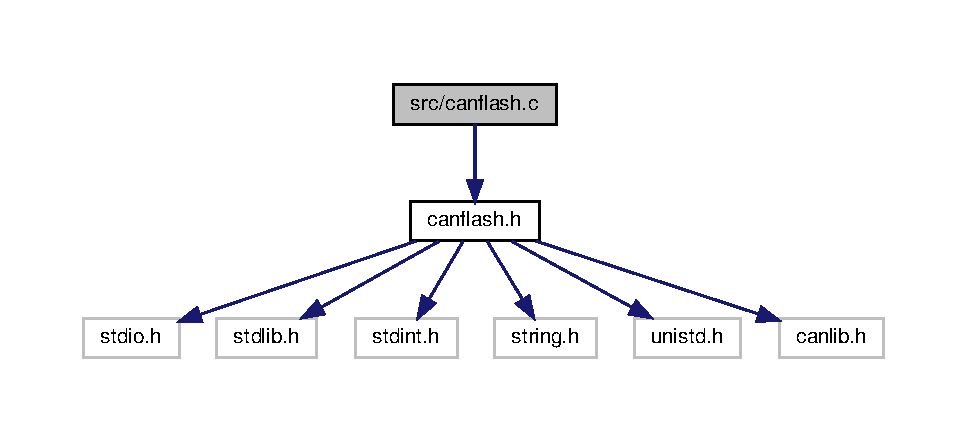
\includegraphics[width=350pt]{canflash_8c__incl}
\end{center}
\end{figure}
\subsection*{Functions}
\begin{DoxyCompactItemize}
\item 
int \hyperlink{canflash_8c_a3c04138a5bfe5d72780bb7e82a18e627}{main} (int argc, char $\ast$$\ast$argv)
\item 
uint8\+\_\+t \hyperlink{canflash_8c_a9284dbafa55fb0f7a9133ed784f55d11}{load\+File} (char $\ast$file\+Path, uint8\+\_\+t $\ast$$\ast$file\+Buffer, uint32\+\_\+t $\ast$file\+Len)
\begin{DoxyCompactList}\small\item\em Loads file from filesystem into given buffer. \end{DoxyCompactList}\item 
\hyperlink{canflash_8h_a470fb8f6490e1526945b47dddbc616c4}{C\+A\+N\+I\+F\+\_\+\+Type\+Def} \hyperlink{canflash_8c_ae4dd3190f91742c0d6916aa0e251981c}{C\+A\+N\+\_\+init} (void)
\begin{DoxyCompactList}\small\item\em Initializes C\+AN interface. \end{DoxyCompactList}\item 
\hyperlink{canflash_8h_a470fb8f6490e1526945b47dddbc616c4}{C\+A\+N\+I\+F\+\_\+\+Type\+Def} \hyperlink{canflash_8c_a54e7a9db928798b80c9b7fd5a4a69f0f}{C\+A\+N\+\_\+tx\+Frame} (uint16\+\_\+t id, uint8\+\_\+t $\ast$frame\+Data, uint8\+\_\+t dlc)
\begin{DoxyCompactList}\small\item\em Transmits data via C\+AN interface. \end{DoxyCompactList}\item 
\hyperlink{canflash_8h_a470fb8f6490e1526945b47dddbc616c4}{C\+A\+N\+I\+F\+\_\+\+Type\+Def} \hyperlink{canflash_8c_a13ff004191c702d4fcd4b8ce43ef7bcb}{C\+A\+N\+\_\+tx\+Data} (uint8\+\_\+t $\ast$file\+Buffer, uint32\+\_\+t $\ast$file\+Len)
\item 
\hyperlink{canflash_8h_a470fb8f6490e1526945b47dddbc616c4}{C\+A\+N\+I\+F\+\_\+\+Type\+Def} \hyperlink{canflash_8c_ac5cef523b584554f39daf8d5e4c10239}{C\+A\+N\+\_\+status\+Handler} (can\+Status can\+Status\+Handler)
\end{DoxyCompactItemize}


\subsection{Function Documentation}
\mbox{\Hypertarget{canflash_8c_ae4dd3190f91742c0d6916aa0e251981c}\label{canflash_8c_ae4dd3190f91742c0d6916aa0e251981c}} 
\index{canflash.\+c@{canflash.\+c}!C\+A\+N\+\_\+init@{C\+A\+N\+\_\+init}}
\index{C\+A\+N\+\_\+init@{C\+A\+N\+\_\+init}!canflash.\+c@{canflash.\+c}}
\subsubsection{\texorpdfstring{C\+A\+N\+\_\+init()}{CAN\_init()}}
{\footnotesize\ttfamily \hyperlink{canflash_8h_a470fb8f6490e1526945b47dddbc616c4}{C\+A\+N\+I\+F\+\_\+\+Type\+Def} C\+A\+N\+\_\+init (\begin{DoxyParamCaption}\item[{void}]{ }\end{DoxyParamCaption})}



Initializes C\+AN interface. 

\begin{DoxyReturn}{Returns}
Returns status as C\+A\+N\+I\+F\+\_\+\+Type\+Def 
\end{DoxyReturn}
\begin{DoxyRefDesc}{Todo}
\item[\hyperlink{todo__todo000001}{Todo}]Add other interfaces as K\+V\+A\+S\+ER leaf light \end{DoxyRefDesc}
\mbox{\Hypertarget{canflash_8c_ac5cef523b584554f39daf8d5e4c10239}\label{canflash_8c_ac5cef523b584554f39daf8d5e4c10239}} 
\index{canflash.\+c@{canflash.\+c}!C\+A\+N\+\_\+status\+Handler@{C\+A\+N\+\_\+status\+Handler}}
\index{C\+A\+N\+\_\+status\+Handler@{C\+A\+N\+\_\+status\+Handler}!canflash.\+c@{canflash.\+c}}
\subsubsection{\texorpdfstring{C\+A\+N\+\_\+status\+Handler()}{CAN\_statusHandler()}}
{\footnotesize\ttfamily \hyperlink{canflash_8h_a470fb8f6490e1526945b47dddbc616c4}{C\+A\+N\+I\+F\+\_\+\+Type\+Def} C\+A\+N\+\_\+status\+Handler (\begin{DoxyParamCaption}\item[{can\+Status}]{can\+Status\+Handler }\end{DoxyParamCaption})}

\mbox{\Hypertarget{canflash_8c_a13ff004191c702d4fcd4b8ce43ef7bcb}\label{canflash_8c_a13ff004191c702d4fcd4b8ce43ef7bcb}} 
\index{canflash.\+c@{canflash.\+c}!C\+A\+N\+\_\+tx\+Data@{C\+A\+N\+\_\+tx\+Data}}
\index{C\+A\+N\+\_\+tx\+Data@{C\+A\+N\+\_\+tx\+Data}!canflash.\+c@{canflash.\+c}}
\subsubsection{\texorpdfstring{C\+A\+N\+\_\+tx\+Data()}{CAN\_txData()}}
{\footnotesize\ttfamily \hyperlink{canflash_8h_a470fb8f6490e1526945b47dddbc616c4}{C\+A\+N\+I\+F\+\_\+\+Type\+Def} C\+A\+N\+\_\+tx\+Data (\begin{DoxyParamCaption}\item[{uint8\+\_\+t $\ast$}]{file\+Buffer,  }\item[{uint32\+\_\+t $\ast$}]{file\+Len }\end{DoxyParamCaption})}

\mbox{\Hypertarget{canflash_8c_a54e7a9db928798b80c9b7fd5a4a69f0f}\label{canflash_8c_a54e7a9db928798b80c9b7fd5a4a69f0f}} 
\index{canflash.\+c@{canflash.\+c}!C\+A\+N\+\_\+tx\+Frame@{C\+A\+N\+\_\+tx\+Frame}}
\index{C\+A\+N\+\_\+tx\+Frame@{C\+A\+N\+\_\+tx\+Frame}!canflash.\+c@{canflash.\+c}}
\subsubsection{\texorpdfstring{C\+A\+N\+\_\+tx\+Frame()}{CAN\_txFrame()}}
{\footnotesize\ttfamily \hyperlink{canflash_8h_a470fb8f6490e1526945b47dddbc616c4}{C\+A\+N\+I\+F\+\_\+\+Type\+Def} C\+A\+N\+\_\+tx\+Frame (\begin{DoxyParamCaption}\item[{uint16\+\_\+t}]{id,  }\item[{uint8\+\_\+t $\ast$}]{frame\+Data,  }\item[{uint8\+\_\+t}]{dlc }\end{DoxyParamCaption})}



Transmits data via C\+AN interface. 


\begin{DoxyParams}[1]{Parameters}
\mbox{\tt in}  & {\em id} & ID of C\+AN message \\
\hline
\mbox{\tt in}  & {\em frame\+Data} & Data to transmit via C\+AN \\
\hline
\mbox{\tt in}  & {\em dlc} & Data Length Code of C\+AN message, also length of frame\+Data \\
\hline
\end{DoxyParams}
\begin{DoxyReturn}{Returns}
Returns C\+A\+N\+I\+F\+\_\+\+Typ\+Def 
\end{DoxyReturn}
\mbox{\Hypertarget{canflash_8c_a9284dbafa55fb0f7a9133ed784f55d11}\label{canflash_8c_a9284dbafa55fb0f7a9133ed784f55d11}} 
\index{canflash.\+c@{canflash.\+c}!load\+File@{load\+File}}
\index{load\+File@{load\+File}!canflash.\+c@{canflash.\+c}}
\subsubsection{\texorpdfstring{load\+File()}{loadFile()}}
{\footnotesize\ttfamily uint8\+\_\+t load\+File (\begin{DoxyParamCaption}\item[{char $\ast$}]{file\+Path,  }\item[{uint8\+\_\+t $\ast$$\ast$}]{file\+Buffer,  }\item[{uint32\+\_\+t $\ast$}]{file\+Len }\end{DoxyParamCaption})}



Loads file from filesystem into given buffer. 


\begin{DoxyParams}[1]{Parameters}
\mbox{\tt in}  & {\em file\+Path} & Pointer to string with path of file to load into buffer \\
\hline
\mbox{\tt out}  & {\em file\+Buffer} & Pointer to buffer to load file to \\
\hline
\mbox{\tt out}  & {\em file\+Len} & Pointer to uint32\+\_\+t for size of loaded file \\
\hline
\end{DoxyParams}
\begin{DoxyReturn}{Returns}
Returns 0 if loading failes, returns 1 if loading succeded 
\end{DoxyReturn}
\mbox{\Hypertarget{canflash_8c_a3c04138a5bfe5d72780bb7e82a18e627}\label{canflash_8c_a3c04138a5bfe5d72780bb7e82a18e627}} 
\index{canflash.\+c@{canflash.\+c}!main@{main}}
\index{main@{main}!canflash.\+c@{canflash.\+c}}
\subsubsection{\texorpdfstring{main()}{main()}}
{\footnotesize\ttfamily int main (\begin{DoxyParamCaption}\item[{int}]{argc,  }\item[{char $\ast$$\ast$}]{argv }\end{DoxyParamCaption})}


%--- End generated contents ---

% Index
\backmatter
\newpage
\phantomsection
\clearemptydoublepage
\addcontentsline{toc}{chapter}{Index}
\printindex

\end{document}
